	\section{Veje}
Vi har indtil videre snakket om knuder, og hvordan de som knudersæt forbindes med kanter. I dette afsnit vil vi udvide det til at snakke om veje, som er sekvenser af disse kanter. Hvis der er tale om ikke-orienterede grafer, er veje defineret ved:
\begin{defn}
[Veje] 
Lad $n \in \N _0$  og $G$ være en ikke-orienteret graf. En vej af længde $n$, fra $u$ til $v$, i $G$ er en sekvens af $n$ kanter $e_{1},e_{2},\cdots,e_{n}$ for $G$, for hvilket der eksisterer en sekvens, $x_{0}=u$ og $x_{1},x_{2},\cdots,x_{n-1}$,$x_{n}=v$, af knuder sådan at $e_{i}$ har, for $i=1,2,\cdots,n$, endeknudererne $x_{i-1}$ og $x_{i}$. Når grafen er simpel, betegnes vejen ved dens knudesekvens $x_{o},x_{1},\cdots,x_{n}$. Vejen passeret igennem knuderne $x_{o},x_{1},\cdots,x_{n-1}$ eller krydse kanterne $e_{1},e_{2},\cdots,e_{n}$. En vej er simpel, hvis den ikke krydser den samme kant mere end én gang.
\end{defn}
Kigger vi derimod på veje med orienterede grafer, som er det vi beskæftiger os med i problemet, ser definitionen en smule anderledes ud:
\begin{defn}
[Veje] 
Lad $n \in \N _0$ og $G$ være en orienteret graf. En vej af længde $n$ fra $u$ til $v$ i $G$ er en sekvens af kanter $e_{1},e_{2},\cdots,e_{n}$ for $G$, sådan at $e_{1}$ er forbundet med $(x_{0},x_{1})$, $e_{2}$ er forbundet med $(x_{1},x_{2})$ og så videre frem til $e_{n}$, som er forbundet med $(x_{n-1},x_{n})$. Her er $x_{0}=u$ og $x_{n}=v$. Hvis alle knudesæt er forbundet med højst én kant per sæt, betegner vi denne  vej ved dets knudesekvens $x_{o},x_{1},\cdots,x_{n}$. En vej er simpel, hvis den ikke krydser den samme kant mere end én gang.
\end{defn}

\begin{figure}[H]
\centering
	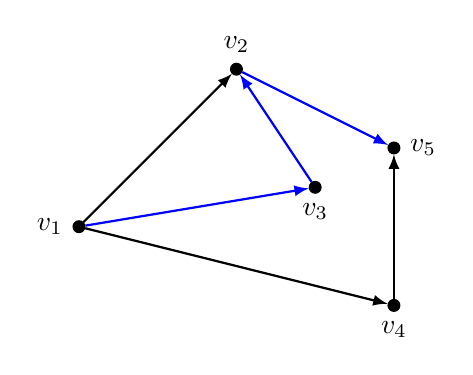
\begin{tikzpicture}

      \tikzset{enclosed/.style={draw, circle, inner sep=0pt, minimum size=.15cm, fill=black}}
%% Vertices
      	\node[enclosed, label={left: $v_1$}] (v1) at (0,2) {};
      	\node[enclosed, label={below: $v_3$}] (v2) at (3,2.5) {};
    		\node[enclosed, label={below: $v_4$}] (v3) at (4,1) {};
  	    \node[enclosed, label={above: $v_2$}] (v4) at (2,4) {};
     	\node[enclosed, label={right: $v_5$}] (v5) at (4,3) {};
%Edges
		\path [->, >=latex, thick, blue](v1) edge node[midway, sloped, above] {} (v2);
		\path [->, >=latex, thick](v1) edge node[midway, sloped, above] {} (v3);
		\path [->, >=latex, thick](v1) edge node[midway, above] {} (v4);
		\path [->, >=latex, thick, blue](v2) edge node[near end, sloped, below] {} (v4);
		\path [->, >=latex, thick](v3) edge node[midway, below] {} (v5);
		\path [->, >=latex, thick, blue](v4) edge node[near end, sloped, above] {} (v5);

	\end{tikzpicture}
	\caption{Eksempel på en orienteret simpel graf og en vej fra $v_{1}$ til $v_{5}$}
	\label{fig.vaegtetopg}
\end{figure}

Antallet af veje mellem to knuder i grafen kan findes ved hjælp af nabomatricer, som vi diskuterede i forrige afsnit.
\begin{thm}
[Antallet af veje mellem to knuder] 
Lad G være en vilkårlig graf med nabomatricen
\textbf{$A$} med grafens knuder i rækkefølgen $v_{1},v_{2},\cdots,v_{n}$. Antallet af forskellige veje med længde $r$ fra $v_{i}$ til $v_{j}$ vil da være lig den $(i,j)$'te indgang af \textbf{$A^{r}$}.
\end{thm}

\begin{proof}
Bevis: Lad G være en graf med nabomatricen 
\textbf{$A$}, hvor vi antager, at knuderne i $G$ har rækkefølgen $v_{1},v_{2},\cdots,v_{n}$. Antallet af veje fra $v_{i}$ til $v_{j}$ af længde 1 er da den $(i,j)$'te indgang til 
\textbf{$A$}. Dette skyldes, at det blot er antallet af kanter fra $v_{i}$ til $v_{j}$.
Vi antager, at den $(i,j)$'te indgang til 
\textbf{${A^r}$} er antallet af forskellige veje, som går fra $v_{i}$ til $v_{j}$ og som har længden $r$. Dette er hypotesen, vi ønsker at bekræfte.
Vi ser på nabomatricen \textbf{$A^{r+1}$}. 
\textbf{$A^{r+1}$} er det samme som 
\textbf{$A^{r}$}$\cdot$\textbf{$A$}, og derfor er den $(i,j)$'te indgang af \textbf{$A^{r+1}$} lig med $b_{i1}a_{1j} + b_{i2}a_{2j} +\cdots+ b_{in}a_{nj}$. Her er $b_{ik}$  den $(i,k)$'te indgang til 
\textbf{$A^{r}$}, som ifølge vores hypotese er antallet af veje fra $v_{i}$ til $v_{k}$ med længde $r$.
En vej af længde $r + 1$ fra $v_{i}$ til $v_{k}$ er lavet ud fra en vej med længden $r$ fra begyndelsesknuden $v_{i}$ og hen til en mellemliggende knude $v_{k}$ samt den kant, der går fra $v_{k}$ til $v_{j}$. Vi ved fra kombinatorik, at antallet af muligheder er lig produktet af mulighederne ved første udfald og mulighederne ved andet udfald. Vi betegner antallet af veje med længden $r$ fra $v_{i}$ til $v_{k}$ med $b_{ik}$ og antallet af kanter fra $v_{k}$ til $v_{j}$ med $a_{kj}$ Finder vi produktet af dette for alle mellemliggende knuder, $v_{k}$, fås det ønskede resultat.
\end{proof}

\begin{exmp}
Vi starter med at kigge på en graf og den tilhørende nabomatrice:
\begin{figure}[H]
\centering
	\begin{tikzpicture}

      \tikzset{enclosed/.style={draw, circle, inner sep=0pt, minimum size=.15cm, fill=black}}
%% Vertices
      	\node[enclosed, label={left: $v_0$}] (v0) at (1,2) {};
      	\node[enclosed, label={above: $v_1$}] (v1) at (3,4) {};
    	\node[enclosed, label={below: $v_2$}] (v2) at (1,0) {};
  	    \node[enclosed, label={right: $v_3$}] (v3) at (5,2) {};
     	\node[enclosed, label={below: $v_4$}] (v4) at (5,0) {};
%Edges
		\path (v0) edge node[midway, sloped, above] {} (v1);
		\path (v0) edge node[midway, sloped, above] {} (v2);
		\path (v0) edge node[midway, above] {} (v3);
		\path (v1) edge node[near end, sloped, below] {} (v3);
		\path (v2) edge node[midway, below] {} (v4);
		\path (v3) edge node[near end, sloped, above] {} (v4);

	\end{tikzpicture}
	\caption{Eksempel på en ikke-orienteret simpel graf}
	\label{fig.vaegtetopg}
\end{figure}

\begin{equation}
A=\begin{bmatrix}
    0&1&1&1&0\\
    1&0&0&1&0\\
    1&0&0&0&1\\
    1&1&0&0&1\\
    0&0&1&1&0\\
\end{bmatrix}
\end{equation}


Vi ønsker at finde ud af hvor mange veje med en længde på 4, der går fra $v_1$ til $v_5$. Det ses i nabomatricen, at $v_1$ har 3 naboer, nemlig $v_2$, $v_3$ og $v_4$. Fortsætter vi, kan vi se, at $v_2$ har $v_1$ og $v_4$ som naboer, $v_3$ har $v_1$ og $v_5$, og $v_4$ har $v_1$, $v_2$ og $v_5$ som naboer. Fortsætter vi, så vi finder alle tænkelige veje med længder på 3, får vi, at der er 18 forskellige veje, der alle starter i $v_1$ og har en længde på 3. Vi skal nu finde de veje, der ved at tilføje en kant, ender i $v_5$. Vi kan se, at $v_5$ har $v_3$ og $v_4$ som naboer. Vi finder derfor de veje, der starter i $v_1$ og slutter i $v_3$, med længden 3, og derefter dem, der slutter i $v_4$, med længden 3. På denne måde udnytter vi, hvad vi skrev i beviset, nemlig at
\textbf{$A^{r+1}$} er lig med $b_{i1}a_{1j} + b_{i2}a_{2j} +\cdots+ b_{in}a_{nj}$
Her er $b_{ik}$ antallet af veje fra $v_{i}$ til ${v_k}$. I vores eksempel er $v_{i}=v_{1}$, ${v_k}=v_{3}$ og ${v_k}=v_{4}$ og \textbf{$A^{r+1}$}=\textbf{$A^{3+1}$}. 
 
\begin{figure}[H]
\centering
	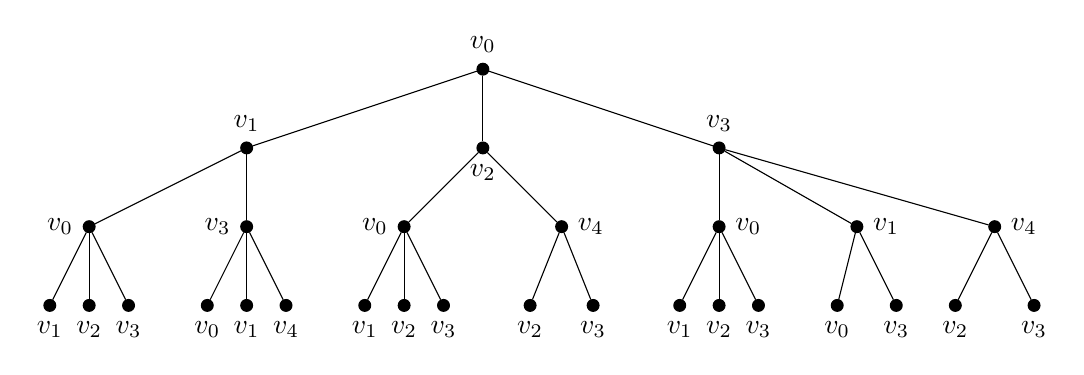
\begin{tikzpicture}

      \tikzset{enclosed/.style={draw, circle, inner sep=0pt, minimum size=.15cm, fill=black}}
%% Vertices
      	\node[enclosed, label={above: $v_0$}] (v0) at (3,6) {};
      	\node[enclosed, label={above: $v_1$}] (v1) at (0,5) {};
    		\node[enclosed, label={below: $v_2$}] (v2) at (3,5) {};
  	    \node[enclosed, label={above: $v_3$}] (v3) at (6,5) {};
     	\node[enclosed, label={left: $v_0$}] (v4) at (-2,4) {};
     	\node[enclosed, label={left: $v_3$}] (v5) at (0,4) {};
     	\node[enclosed, label={left: $v_0$}] (v6) at (2,4) {};
     	\node[enclosed, label={right: $v_4$}] (v7) at (4,4) {};
     	\node[enclosed, label={right: $v_0$}] (v8) at (6,4) {};
     	\node[enclosed, label={right: $v_1$}] (v9) at (7.75,4) {};
     	\node[enclosed, label={right: $v_4$}] (v10) at (9.5,4) {};
     	\node[enclosed, label={below: $v_1$}] (v11) at (-2.5,3) {};
      	\node[enclosed, label={below: $v_2$}] (v12) at (-2,3) {};
  	    \node[enclosed, label={below: $v_3$}] (v13) at (-1.5,3) {};
  	    \node[enclosed, label={below: $v_0$}] (v14) at (-0.5,3) {};
     	\node[enclosed, label={below: $v_1$}] (v15) at (0,3) {};
     	\node[enclosed, label={below: $v_4$}] (v16) at (0.5,3) {};
     	\node[enclosed, label={below: $v_1$}] (v17) at (1.5,3) {};
      	\node[enclosed, label={below: $v_2$}] (v18) at (2,3) {};
  	    \node[enclosed, label={below: $v_3$}] (v19) at (2.5,3) {};
  	    \node[enclosed, label={below: $v_2$}] (v20) at (3.6,3) {};
  	    \node[enclosed, label={below: $v_3$}] (v21) at (4.4,3) {};
  	    \node[enclosed, label={below: $v_1$}] (v22) at (5.5,3) {};
      	\node[enclosed, label={below: $v_2$}] (v23) at (6,3) {};
  	    \node[enclosed, label={below: $v_3$}] (v24) at (6.5,3) {};
  	    \node[enclosed, label={below: $v_0$}] (v25) at (7.5,3) {};
     	\node[enclosed, label={below: $v_3$}] (v26) at (8.25,3) {};
     	\node[enclosed, label={below: $v_2$}] (v27) at (9,3) {};
     	\node[enclosed, label={below: $v_3$}] (v28) at (10,3) {};
%Edges
		\path (v0) edge node[midway, sloped, above] {} (v1);
		\path (v0) edge node[midway, sloped, above] {} (v2);
		\path (v0) edge node[midway, above] {} (v3);
		\path (v1) edge node[near end, sloped, below] {} (v4);
		\path (v1) edge node[midway, below] {} (v5);
		\path (v2) edge node[near end, sloped, above] {} (v6);
		\path (v2) edge node[near end, sloped, above] {} (v7);
		\path (v3) edge node[near end, sloped, above] {} (v8);
		\path (v3) edge node[near end, sloped, above] {} (v9);
		\path (v3) edge node[near end, sloped, above] {} (v10);
		\path (v4) edge node[near end, sloped, above] {} (v11);
		\path (v4) edge node[near end, sloped, above] {} (v12);
		\path (v4) edge node[near end, sloped, above] {} (v13);
		\path (v5) edge node[near end, sloped, above] {} (v14);
		\path (v5) edge node[near end, sloped, above] {} (v15);
		\path (v5) edge node[near end, sloped, above] {} (v16);
		\path (v6) edge node[near end, sloped, above] {} (v17);
		\path (v6) edge node[near end, sloped, above] {} (v18);
		\path (v6) edge node[near end, sloped, above] {} (v19);
		\path (v7) edge node[near end, sloped, above] {} (v20);
		\path (v7) edge node[near end, sloped, above] {} (v21);
		\path (v8) edge node[near end, sloped, above] {} (v22);
		\path (v8) edge node[near end, sloped, above] {} (v23);
		\path (v8) edge node[near end, sloped, above] {} (v24);
		\path (v9) edge node[near end, sloped, above] {} (v25);
		\path (v9) edge node[near end, sloped, above] {} (v26);
		\path (v10) edge node[near end, sloped, above] {} (v27);
		\path (v10) edge node[near end, sloped, above] {} (v28);

	\end{tikzpicture}
	\caption{De mulige løsninger for veje med længde 3 fra $v_{0}$ til $v_{k}$}
	\label{fig.vaegtetopg}
\end{figure}

Antallet af veje fra $v_{1}$ til $v_{3}$ er 5, og antallet af veje fra $v_{1}$ til $v_{4}$ er 6. Vi kan derfor opstille
\textbf{$A^{4}$}$=b_{1i} \cdot a_{1j}+b_{2i} \cdot a_{2j}=5 \cdot 1+6 \cdot 1=11$.
Her er $b_{1i}$ antallet af veje fra $v_{i}=v_{1}$ til vores første $v_{k}=v_{3}$, og $a_{1j}$ er antallet af kanter fra første $v_{k}=v_{3}$ til  $v_{j}=v_{5}$. På samme måde optræder $b_{2i}$ og $a_{2j}$ for vores andet $v_{k}=v_{4}$. Der er altså 11 veje med længden 4 fra knuden $v_{1}$ til knuden $v_{5}$.

\end{exmp}

\subsection{Vægtede grafer}
En \emph{vægtet graf} er en graf, hvori kanterne eller knuderne får tildelt en numerisk værdi. I dette projekt arbejdes der udelukkende med vægtede kanter, og vi vil derfor kun fokusere på dem i dette afsnit.
En vægtet graf er defineret ved:
\begin{defn}[Vægtede grafer]
En vægtet graf, $G=(V,E,w)$, består af en mængde knuder, $V$, en mængde kanter, $E$, og \emph{vægtfunktionen}, $w: E \rightarrow \R$.
\end{defn}

For en vægtet graf har alle kanter $e\in E$ en numerisk vægt, givet ved funktionen $w (e)$. Da $e$ er en kant incident med $\{u,v\}$ kan man ligeledes skrive $w (u,v)$. På samme måde som med uvægtede grafer, kan en vægtet graf også opdeles i de seks graftyper fundet i tabel \ref{tab:typer}.
\begin{figure}[H]
\centering
	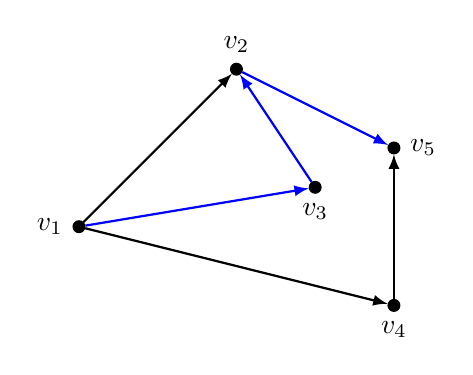
\begin{tikzpicture}

      \tikzset{enclosed/.style={draw, circle, inner sep=0pt, minimum size=.15cm, fill=black}}
%% Vertices
      	\node[enclosed, label={left: $v_1$}] (v1) at (0,2) {};
      	\node[enclosed, label={below: $v_3$}] (v2) at (3,2.5) {};
    		\node[enclosed, label={below: $v_4$}] (v3) at (4,1) {};
  	    \node[enclosed, label={above: $v_2$}] (v4) at (2,4) {};
     	\node[enclosed, label={right: $v_5$}] (v5) at (4,3) {};
%Edges
		\path [->, >=latex, thick, blue](v1) edge node[midway, sloped, above] {} (v2);
		\path [->, >=latex, thick](v1) edge node[midway, sloped, above] {} (v3);
		\path [->, >=latex, thick](v1) edge node[midway, above] {} (v4);
		\path [->, >=latex, thick, blue](v2) edge node[near end, sloped, below] {} (v4);
		\path [->, >=latex, thick](v3) edge node[midway, below] {} (v5);
		\path [->, >=latex, thick, blue](v4) edge node[near end, sloped, above] {} (v5);

	\end{tikzpicture}
	\caption{Eksempel på en orienteret simpel graf og en vej fra $v_{1}$ til $v_{5}$}
	\label{fig.vaegtetopg}
\end{figure}

Da vægtede grafer har en numerisk vægt på hver kant, kan man således beregne \emph{distancen} fra en knude til en anden i grafen. Distancen fra en knude til en anden kan defineres således:

\begin{defn}[Distance]
Lad $m\in \N $, $G=(V,E,w)$ være en vilkårlig graf og  $e_{v_i,v_{i+1}}$ være en kant, som er incident med $v_i$ og $v_{i+1}$. Lad en tilfældig, simpel vej, $P$, gå igennem knuderne således $P=(v_{1},v_{2},\dotsc,v_{m})$, da kan distancen beskrives som
	\begin{equation*}
	\mathrm{dist}(P)=\sum_{i=1}^{m}w(e_{v_i,v_{i+1}}).
	\end{equation*}  
\end{defn}

Man kan således bruge følgende definitioner af \emph{korteste vej} og \emph{længste vej} i en vægtet graf:


\begin{defn} [Korteste vej i vægtet graf]\label{defn:min.vej}
Lad $G=(V,E,w)$ være en vilkårlig, vægtet graf. Da er distancen af den korteste vej, fra en knude, $v_1$, til en anden knude, $v_m$, defineret som
	\begin{equation*}
		\alpha(v_1,v_m)=\arg \min_{P \in \euscr{P}}
		\textrm{dist}(P),
	\end{equation*}
	hvor $\euscr{P}$ er mængden af alle veje fra $v_1$ til $v_m$.
\end{defn}

På samme vis defineres længste vej:

\begin{defn} [Længste vej i en vægtet graf]
	Lad $G=(V,E,w)$ være en vilkårlig, vægtet graf. Da er distancen af den længste vej, fra en knude, $v_1$, til en anden knude, $v_m$, defineret som
	\begin{equation*}
		\beta(v_1,v_m)=\arg \max_{P \in \euscr{P}}
		\textrm{dist}(P),
	\end{equation*}
	hvor $\euscr{P}$ er mængden af alle veje fra $v_1$ til $v_m$.
\end{defn}

\begin{exmp}
Betragt figur \ref{fig.vaegtetopg} \\
\begin{figure}[H]
\centering
	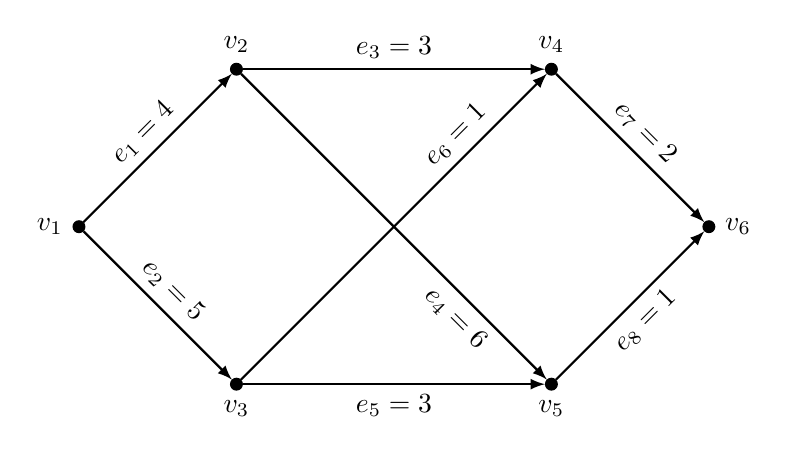
\begin{tikzpicture}

      \tikzset{enclosed/.style={draw, circle, inner sep=0pt, minimum size=.15cm, fill=black}}
%% Vertices
      	\node[enclosed, label={left: $v_1$}] (v1) at (0,2) {};
      	\node[enclosed, label={above: $v_2$}] (v2) at (2,4) {};
    	\node[enclosed, label={below: $v_3$}] (v3) at (2,0) {};
  	    \node[enclosed, label={above: $v_4$}] (v4) at (6,4) {};
     	\node[enclosed, label={below: $v_5$}] (v5) at (6,0) {};
     	\node[enclosed, label={right: $v_6$}] (v6) at (8,2) {};
%Edges
		\path [->, > = latex, thick] (v1) edge node[midway, sloped, above] {$e_1=4$} (v2);
		\path [->, > = latex, thick] (v1) edge node[midway, sloped, above] {$e_2=5$} (v3);
		\path [->, > = latex, thick] (v2) edge node[midway, above] {$e_3=3$} (v4);
		\path [->, > = latex, thick] (v2) edge node[near end, sloped, below] {$e_4=6$} (v5);
		\path [->, > = latex, thick] (v3) edge node[midway, below] {$e_5=3$} (v5);
		\path [->, > = latex, thick] (v3) edge node[near end, sloped, above] {$e_6=1$} (v4);
		\path [->, > = latex, thick] (v4) edge node[midway, sloped, above] {$e_7=2$} (v6);
		\path [->, > = latex, thick] (v5) edge node[midway, sloped, below] {$e_8=1$} (v6);

	\end{tikzpicture}
	\caption{En simpel, orienteret og vægtet graf.}
	\label{fig.vaegtetopg}
\end{figure}


På figuren ses en graf med vægtede kanter. Vi er interesserede i at finde den korteste vej fra $v_1$ til $v_6$. For at finde den korteste vej, kigger vi på alle de mulige veje fra $v_1$ til $v_6$.
Følgende veje ses:
\begin{align*}
	P_1=&(v_1,v_2,v_4,v_6)\\
	P_2=&(v_1,v_2,v_5,v_6)\\
	P_3=&(v_1,v_3,v_5,v_6)\\
	P_4=&(v_1,v_3,v_4,v_6)
\end{align*}
Man kan nu beregne distancen af de fire veje, ved at tage summen af de kanter, vejen følger. Man får derved:
\begin{align*}
	P_1=&4+3+2=9\\
	P_2=&4+6+1=11\\
	P_3=&5+3+1=9\\
	P_4=&5+1+2=8
\end{align*}
Det ses, at den korteste vej fra $v_1$ til $v_6$ er $P_4$. 
Det er sådan, man kan finde korteste vej i en vægtet graf. Denne metode kaldes \emph{brute force}. Metoden kan blive meget tidskrævende ved mere komplekse grafer. I disse tilfælde vil man bruge alternative, bedre algoritmer til at løse problemet. Dette vil vi komme ind på senere i kapitel \ref{kap.algo}.
\end{exmp}
